\documentclass{standalone}
\usepackage{tikz}
\usetikzlibrary{patterns, positioning}


\begin{document}
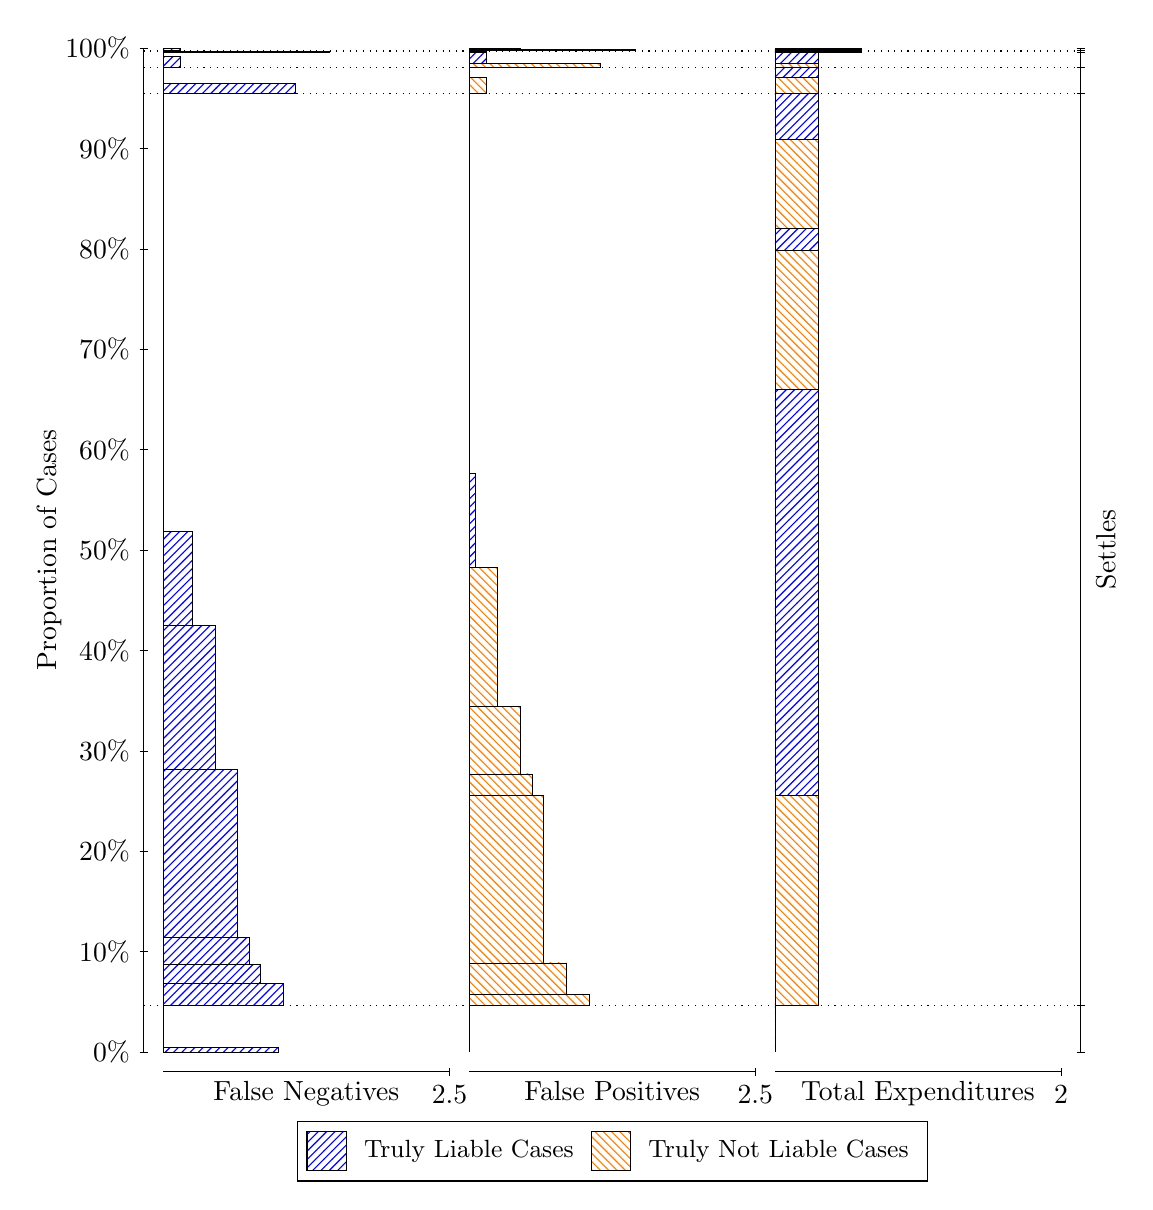
\begin{tikzpicture}
\draw[black, very thin] (1.5,1.75) -- (1.5,14.5);
\node[rotate=90, text=black, anchor=center] at (0.3, 8.125) {Proportion of Cases};
\draw[black, very thin] (1.45,1.75) -- (1.55,1.75);
\node[text=black, anchor=east] at (1.45, 1.75) {0\%};
\draw[black, very thin] (1.45,3.025) -- (1.55,3.025);
\node[text=black, anchor=east] at (1.45, 3.025) {10\%};
\draw[black, very thin] (1.45,4.3) -- (1.55,4.3);
\node[text=black, anchor=east] at (1.45, 4.3) {20\%};
\draw[black, very thin] (1.45,5.575) -- (1.55,5.575);
\node[text=black, anchor=east] at (1.45, 5.575) {30\%};
\draw[black, very thin] (1.45,6.85) -- (1.55,6.85);
\node[text=black, anchor=east] at (1.45, 6.85) {40\%};
\draw[black, very thin] (1.45,8.125) -- (1.55,8.125);
\node[text=black, anchor=east] at (1.45, 8.125) {50\%};
\draw[black, very thin] (1.45,9.4) -- (1.55,9.4);
\node[text=black, anchor=east] at (1.45, 9.4) {60\%};
\draw[black, very thin] (1.45,10.675) -- (1.55,10.675);
\node[text=black, anchor=east] at (1.45, 10.675) {70\%};
\draw[black, very thin] (1.45,11.95) -- (1.55,11.95);
\node[text=black, anchor=east] at (1.45, 11.95) {80\%};
\draw[black, very thin] (1.45,13.225) -- (1.55,13.225);
\node[text=black, anchor=east] at (1.45, 13.225) {90\%};
\draw[black, very thin] (1.45,14.5) -- (1.55,14.5);
\node[text=black, anchor=east] at (1.45, 14.5) {100\%};

\draw[black, very thin] (13.4,1.75) -- (13.4,14.5);
\draw[black, very thin] (13.35,1.75) -- (13.45,1.75);
\node[anchor=west] at (13.35, 1.75) {};
\draw[black, very thin] (13.35,2.3431) -- (13.45,2.3431);
\node[anchor=west] at (13.35, 2.3431) {};
\draw[black, very thin] (13.35,13.925) -- (13.45,13.925);
\node[anchor=west] at (13.35, 13.925) {};
\draw[black, very thin] (13.35,14.254) -- (13.45,14.254);
\node[anchor=west] at (13.35, 14.254) {};
\draw[black, very thin] (13.35,14.452) -- (13.45,14.452);
\node[anchor=west] at (13.35, 14.452) {};
\draw[black, very thin] (13.35,14.473) -- (13.45,14.473);
\node[anchor=west] at (13.35, 14.473) {};
\draw[black, very thin] (13.35,14.5) -- (13.45,14.5);
\node[anchor=west] at (13.35, 14.5) {};

\draw[black, very thin, pattern color=blue, pattern=north east lines] (1.75,1.75) rectangle (3.2033,1.8124);
\draw[black, very thin, pattern color=orange, pattern=north west lines] (1.75,1.8124) rectangle (1.75,2.3431);
\draw[black, very thin, pattern color=blue, pattern=north east lines] (1.75,2.3431) rectangle (3.276,2.6198);
\draw[black, very thin, pattern color=blue, pattern=north east lines] (1.75,2.6198) rectangle (2.9853,2.8642);
\draw[black, very thin, pattern color=blue, pattern=north east lines] (1.75,2.8642) rectangle (2.84,3.2089);
\draw[black, very thin, pattern color=blue, pattern=north east lines] (1.75,3.2089) rectangle (2.6947,5.3373);
\draw[black, very thin, pattern color=blue, pattern=north east lines] (1.75,5.3373) rectangle (2.404,7.1681);
\draw[black, very thin, pattern color=blue, pattern=north east lines] (1.75,7.1681) rectangle (2.1133,8.3622);
\draw[black, very thin, pattern color=orange, pattern=north west lines] (1.75,8.3622) rectangle (1.75,13.925);
\draw[black, very thin, pattern color=blue, pattern=north east lines] (1.75,13.925) rectangle (3.4213,14.048);
\draw[black, very thin, pattern color=orange, pattern=north west lines] (1.75,14.048) rectangle (1.75,14.254);
\draw[black, very thin, pattern color=blue, pattern=north east lines] (1.75,14.254) rectangle (1.968,14.398);
\draw[black, very thin, pattern color=orange, pattern=north west lines] (1.75,14.398) rectangle (1.75,14.452);
\draw[black, very thin, pattern color=blue, pattern=north east lines] (1.75,14.452) rectangle (3.8573,14.46);
\draw[black, very thin, pattern color=orange, pattern=north west lines] (1.75,14.46) rectangle (1.75,14.473);
\draw[black, very thin, pattern color=blue, pattern=north east lines] (1.75,14.473) rectangle (1.968,14.492);
\draw[black, very thin, pattern color=orange, pattern=north west lines] (1.75,14.492) rectangle (1.75,14.5);
\draw[black, very thin, pattern color=orange, pattern=north west lines] (5.6333,1.75) rectangle (5.6333,2.2807);
\draw[black, very thin, pattern color=blue, pattern=north east lines] (5.6333,2.2807) rectangle (5.6333,2.3431);
\draw[black, very thin, pattern color=orange, pattern=north west lines] (5.6333,2.3431) rectangle (7.1593,2.4846);
\draw[black, very thin, pattern color=orange, pattern=north west lines] (5.6333,2.4846) rectangle (6.8687,2.8814);
\draw[black, very thin, pattern color=orange, pattern=north west lines] (5.6333,2.8814) rectangle (6.578,5.0099);
\draw[black, very thin, pattern color=orange, pattern=north west lines] (5.6333,5.0099) rectangle (6.4327,5.2816);
\draw[black, very thin, pattern color=orange, pattern=north west lines] (5.6333,5.2816) rectangle (6.2873,6.139);
\draw[black, very thin, pattern color=orange, pattern=north west lines] (5.6333,6.139) rectangle (5.9967,7.9059);
\draw[black, very thin, pattern color=blue, pattern=north east lines] (5.6333,7.9059) rectangle (5.706,9.1);
\draw[black, very thin, pattern color=blue, pattern=north east lines] (5.6333,9.1) rectangle (5.6333,13.925);
\draw[black, very thin, pattern color=orange, pattern=north west lines] (5.6333,13.925) rectangle (5.8513,14.131);
\draw[black, very thin, pattern color=blue, pattern=north east lines] (5.6333,14.131) rectangle (5.6333,14.254);
\draw[black, very thin, pattern color=orange, pattern=north west lines] (5.6333,14.254) rectangle (7.3047,14.308);
\draw[black, very thin, pattern color=blue, pattern=north east lines] (5.6333,14.308) rectangle (5.8513,14.452);
\draw[black, very thin, pattern color=orange, pattern=north west lines] (5.6333,14.452) rectangle (5.8513,14.465);
\draw[black, very thin, pattern color=blue, pattern=north east lines] (5.6333,14.465) rectangle (5.6333,14.473);
\draw[black, very thin, pattern color=orange, pattern=north west lines] (5.6333,14.473) rectangle (7.7407,14.481);
\draw[black, very thin, pattern color=blue, pattern=north east lines] (5.6333,14.481) rectangle (6.2873,14.5);
\draw[black, very thin, pattern color=orange, pattern=north west lines] (9.5167,1.75) rectangle (9.5167,2.2807);
\draw[black, very thin, pattern color=blue, pattern=north east lines] (9.5167,2.2807) rectangle (9.5167,2.3431);
\draw[black, very thin, pattern color=orange, pattern=north west lines] (9.5167,2.3431) rectangle (10.062,5.0099);
\draw[black, very thin, pattern color=blue, pattern=north east lines] (9.5167,5.0099) rectangle (10.062,10.163);
\draw[black, very thin, pattern color=orange, pattern=north west lines] (9.5167,10.163) rectangle (10.062,11.93);
\draw[black, very thin, pattern color=blue, pattern=north east lines] (9.5167,11.93) rectangle (10.062,12.207);
\draw[black, very thin, pattern color=orange, pattern=north west lines] (9.5167,12.207) rectangle (10.062,13.336);
\draw[black, very thin, pattern color=blue, pattern=north east lines] (9.5167,13.336) rectangle (10.062,13.925);
\draw[black, very thin, pattern color=orange, pattern=north west lines] (9.5167,13.925) rectangle (10.062,14.131);
\draw[black, very thin, pattern color=blue, pattern=north east lines] (9.5167,14.131) rectangle (10.062,14.254);
\draw[black, very thin, pattern color=orange, pattern=north west lines] (9.5167,14.254) rectangle (10.062,14.308);
\draw[black, very thin, pattern color=blue, pattern=north east lines] (9.5167,14.308) rectangle (10.062,14.452);
\draw[black, very thin, pattern color=orange, pattern=north west lines] (9.5167,14.452) rectangle (10.607,14.465);
\draw[black, very thin, pattern color=blue, pattern=north east lines] (9.5167,14.465) rectangle (10.607,14.473);
\draw[black, very thin, pattern color=orange, pattern=north west lines] (9.5167,14.473) rectangle (10.607,14.481);
\draw[black, very thin, pattern color=blue, pattern=north east lines] (9.5167,14.481) rectangle (10.607,14.5);
\draw[black, dotted] (1.5,2.3431) -- (13.4,2.3431);
\draw[black, dotted] (1.5,13.925) -- (13.4,13.925);
\draw[black, dotted] (1.5,14.254) -- (13.4,14.254);
\draw[black, dotted] (1.5,14.452) -- (13.4,14.452);
\draw[black, dotted] (1.5,14.473) -- (13.4,14.473);
\draw[black, very thin] (1.75,1.5) -- (5.3833,1.5);
\node[text=black, anchor=north] at (3.5667, 1.5) {False Negatives};
\draw[black, very thin] (5.3833,1.45) -- (5.3833,1.55);
\node[text=black, anchor=north] at (5.3833, 1.45) {2.5};

\draw[black, very thin] (5.6333,1.5) -- (9.2667,1.5);
\node[text=black, anchor=north] at (7.45, 1.5) {False Positives};
\draw[black, very thin] (9.2667,1.45) -- (9.2667,1.55);
\node[text=black, anchor=north] at (9.2667, 1.45) {2.5};

\draw[black, very thin] (9.5167,1.5) -- (13.15,1.5);
\node[text=black, anchor=north] at (11.333, 1.5) {Total Expenditures};
\draw[black, very thin] (13.15,1.45) -- (13.15,1.55);
\node[text=black, anchor=north] at (13.15, 1.45) {2};


\node[text=black, centered, rotate=90] at (13.72, 8.134) {Settles};





\draw (7.449999999999999,1.5) node[draw=none] (baseCoordinate) {};
\begin{scope}[align=center]
        \matrix[scale=0.5, draw=black, below=0.5cm of baseCoordinate, nodes={draw}, column sep=0.1cm]{
            \node[rectangle, draw, minimum width=0.5cm, minimum height=0.5cm, pattern color=blue, pattern=north east lines] {}; &
            \node[draw=none, font=\small, text=black] (B) {Truly Liable Cases}; &
            \node[rectangle, draw, minimum width=0.5cm, minimum height=0.5cm, pattern color=orange, pattern=north west lines] {}; &
            \node[draw=none, font=\small, text=black] (B) {Truly Not Liable Cases}; \\
            };
\end{scope}

\end{tikzpicture}
\end{document}